%%%%%%%%%%%%%%%%%%%%%%%%%%%%%%%%%%%%%%%%%%%%%%%%%%%%%%%%%%%%%%%%%%%%%%%%%%%%
% Nick Waters's super awesome template for biorXiv submissions

% In memory of Henry, Hermione, and Angus.
% May there be many tasty snails in pufferfish heaven
%%%%%%%%%%%%%%%%%%%%%%%%%%%%%%%%%%%%%%%%%%%%%%%%%%%%%%%%%%%%%%%%%%%%%%%%%%%%
\documentclass[10pt]{article}

\usepackage{geometry}
\geometry{marginparwidth=1cm,a4paper,verbose,tmargin=1.5cm,bmargin=1.5cm,lmargin=1.5cm,rmargin=1.5cm,headheight=0cm,headsep=0cm,footskip=0cm}
\usepackage{cite}
\usepackage{hyperref} % make the references clickable
\setlength\parindent{0pt} % set indent to zero
\setlength{\parskip}{1.2em} % give a bit of space between paragraphs

\bibliographystyle{plain} % citation and bib style
\usepackage{grffile} %for underscores in file names
\usepackage[ruled]{algorithm2e} % for typesetting the riboSeed algorithm
\setlength{\algotitleheightrule}{0pt}
\usepackage{lineno, color} % controls line numbering
\modulolinenumbers[5]  % number every 5th line
% format our line numbers, cause no one likes boring numbers
\renewcommand\linenumberfont{\normalfont\tiny\color{blue}}
\usepackage{booktabs}  % less yucky tables
% nice little thing for table spacing (thanks Markus Püschel)
\newcommand{\ra}[1]{\renewcommand{\arraystretch}{#1}}
\usepackage{multirow} % for some pretty tables with merged cells

% my lined-off abstract
\newenvironment{myabstract}{%
\begin{quote} \baselineskip14pt \rule{.89\textwidth}{1.5pt} \vskip .1cm}
{ \vskip -.10cm \rule{.89\textwidth}{1.5pt} \end{quote}}

% supplementary (essentialy just resets numbering)
\newcommand{\beginsupplement}{%
  \setcounter{table}{0}
  \renewcommand{\thetable}{S\arabic{table}}%
  \setcounter{figure}{0}
  \renewcommand{\thefigure}{S\arabic{figure}}%
}
% pretty thought break
\def \thoughtbr {\begin{center}\noindent\rule{.4\textwidth}{0.4pt}  {\raisebox{-.5ex}{$\sim$}}  \rule{.4\textwidth}{0.4pt}\end{center}}

% \usepackage{graphicx}
\graphicspath{ {../../../NAR_riboSeed/riboFigs/} }  %  set the path to the figures

\usepackage{titlesec} % for adjusting spacing after the section headers
\titlespacing\subsection{0pt}{12pt plus 4pt minus 2pt}{-11pt plus 0pt minus 0pt}
\titlespacing\subsubsection{0pt}{12pt plus 4pt minus 2pt}{-11pt plus 0pt minus 0pt}


%%%%%%%%%%%%%%%%%%%%%%%%%%%%%%%%%%%%%%%%%%%%%%%%%%
% this hack stolen from Stack overflow is a macro to make a \cmmidrule
% for each column.  I added the ".4" spacing to get this to look prettier
%  if you have 5 columns, instead of \midrule, you could use \cmidrules{5}
\makeatletter
\newtoks\MD@cmidrules
\newcommand{\cmidrules}[1]{%
  \noalign{%
    \global\MD@cmidrules={}%
    \toks@={\cmidrule(l{.3\tabcolsep}r{.3\tabcolsep})}%
    \count@=\z@
    \loop\ifnum\count@<#1\relax
      \advance\count@\@ne
      \edef\MD@temp{\the\toks@{\the\count@-\the\count@}}%
      \global\MD@cmidrules\expandafter{\the\expandafter\MD@cmidrules\MD@temp}%
    \repeat
  }%
  \the\MD@cmidrules
}
\makeatother
%%%%%%%%%%%%%%%%%%%%%%%%%%%%%%%%%%%%%%%%%%%%%%%%%%
% from NAR
\let\colrule\midrule
\let\botrule\bottomrule


%%%%  This allows us to set the table font size up top
\usepackage{etoolbox}
\BeforeBeginEnvironment{tabular}{\begin{center}\footnotesize}
\AfterEndEnvironment{tabular}{\end{center}}
%%%%

\def \ttilde {\raisebox{-.5ex}\textasciitilde} % fix for ugly cmodern tilde 20160829

%  format captions
\usepackage[%
    font={small},
    labelfont=bf,
    format=hang,
    format=plain,
    margin=0pt,
    width=0.9\textwidth]{caption}
\usepackage[list=true]{subcaption}  % allow for subfigures with captions
\usepackage{amssymb}  % for checkmark symbols
\usepackage{graphicx}  % trim figures
\usepackage{colortbl}  % adjust table colors
\definecolor{lgray}{gray}{.90}  % line grey
\definecolor{tgray}{gray}{.40}  % text grey
\definecolor{egray}{gray}{.01}  % emphasis grey
\usepackage[yyyymmdd,hhmmss]{datetime} % for timestamp

\title{\fontseries{m}\selectfont riboSeed: leveraging prokaryotic genomic architecture to assemble across ribosomal regions}

\author
{\small Nicholas R. Waters,$^{1,2}$ Florence Abram,$^{1}$ Fiona Brennan,$^{1,3}$ Ashleigh Holmes,$^{4}$ and Leighton Pritchard$^{2\ast}$\\
\\
\normalsize{\textit {$^{1}$Department of Microbiology, School of Natural Sciences, National University of Ireland, Galway, Ireland}}\\
\normalsize{\textit {$^{2}$Information and Computational Sciences, James Hutton Institute, Invergowrie, Dundee DD2 5DA, Scotland}}\\
\normalsize{\textit {$^{3}$Soil and Environmental Microbiology, Environmental Research Centre, Teagasc, Johnstown Castle, Wexford, Ireland}}\\
\normalsize{\textit {$^{4}$Cell and Molecular Sciences, James Hutton Institute, Invergowrie, Dundee DD2 5DA, Scotland}}\\
\\
\footnotesize{$^\ast$To whom correspondence should be addressed: leighton.pritchard@hutton.ac.uk}
}
\date{}

\begin{document}
\baselineskip20pt  % set line spacing; double spacing is 2xfontsize, in this case 11
\maketitle
\vspace*{-1.5cm}
{\begin{center}\footnotesize\date{Compiled: \today ~\currenttime}\end{center}}


\begin{myabstract}
  \input{../../../NAR_riboSeed/main_tex/abstract}
\end{myabstract}

Keywords: genome assembly, ribosome, benchmarking, scaffolding, \textit{de fere novo}

\begin{linenumbers}


\section*{Background}

\input{../../../NAR_riboSeed/main_tex/figncbi}
\input{../../../NAR_riboSeed/main_tex/intro1}
\input{../../../NAR_riboSeed/main_tex/intro2}
\input{../../../NAR_riboSeed/main_tex/tabfinishers}
\input{../../../NAR_riboSeed/main_tex/figsummary}


\section*{Implementation}
\input{../../../NAR_riboSeed/main_tex/usage1}
\input{../../../NAR_riboSeed/main_tex/usage2}
\input{../../../NAR_riboSeed/main_tex/avail}

\section*{Results}

\subsection*{Characteristics of rDNA flanking regions}

\input{../../../NAR_riboSeed/main_tex/figcolientropy}
\input{../../../NAR_riboSeed/main_tex/resentropy}

\subsection*{Simulated reads with artificial chromosome}

\begin{figure}[!b]
    \centering
    \hspace*{-2cm}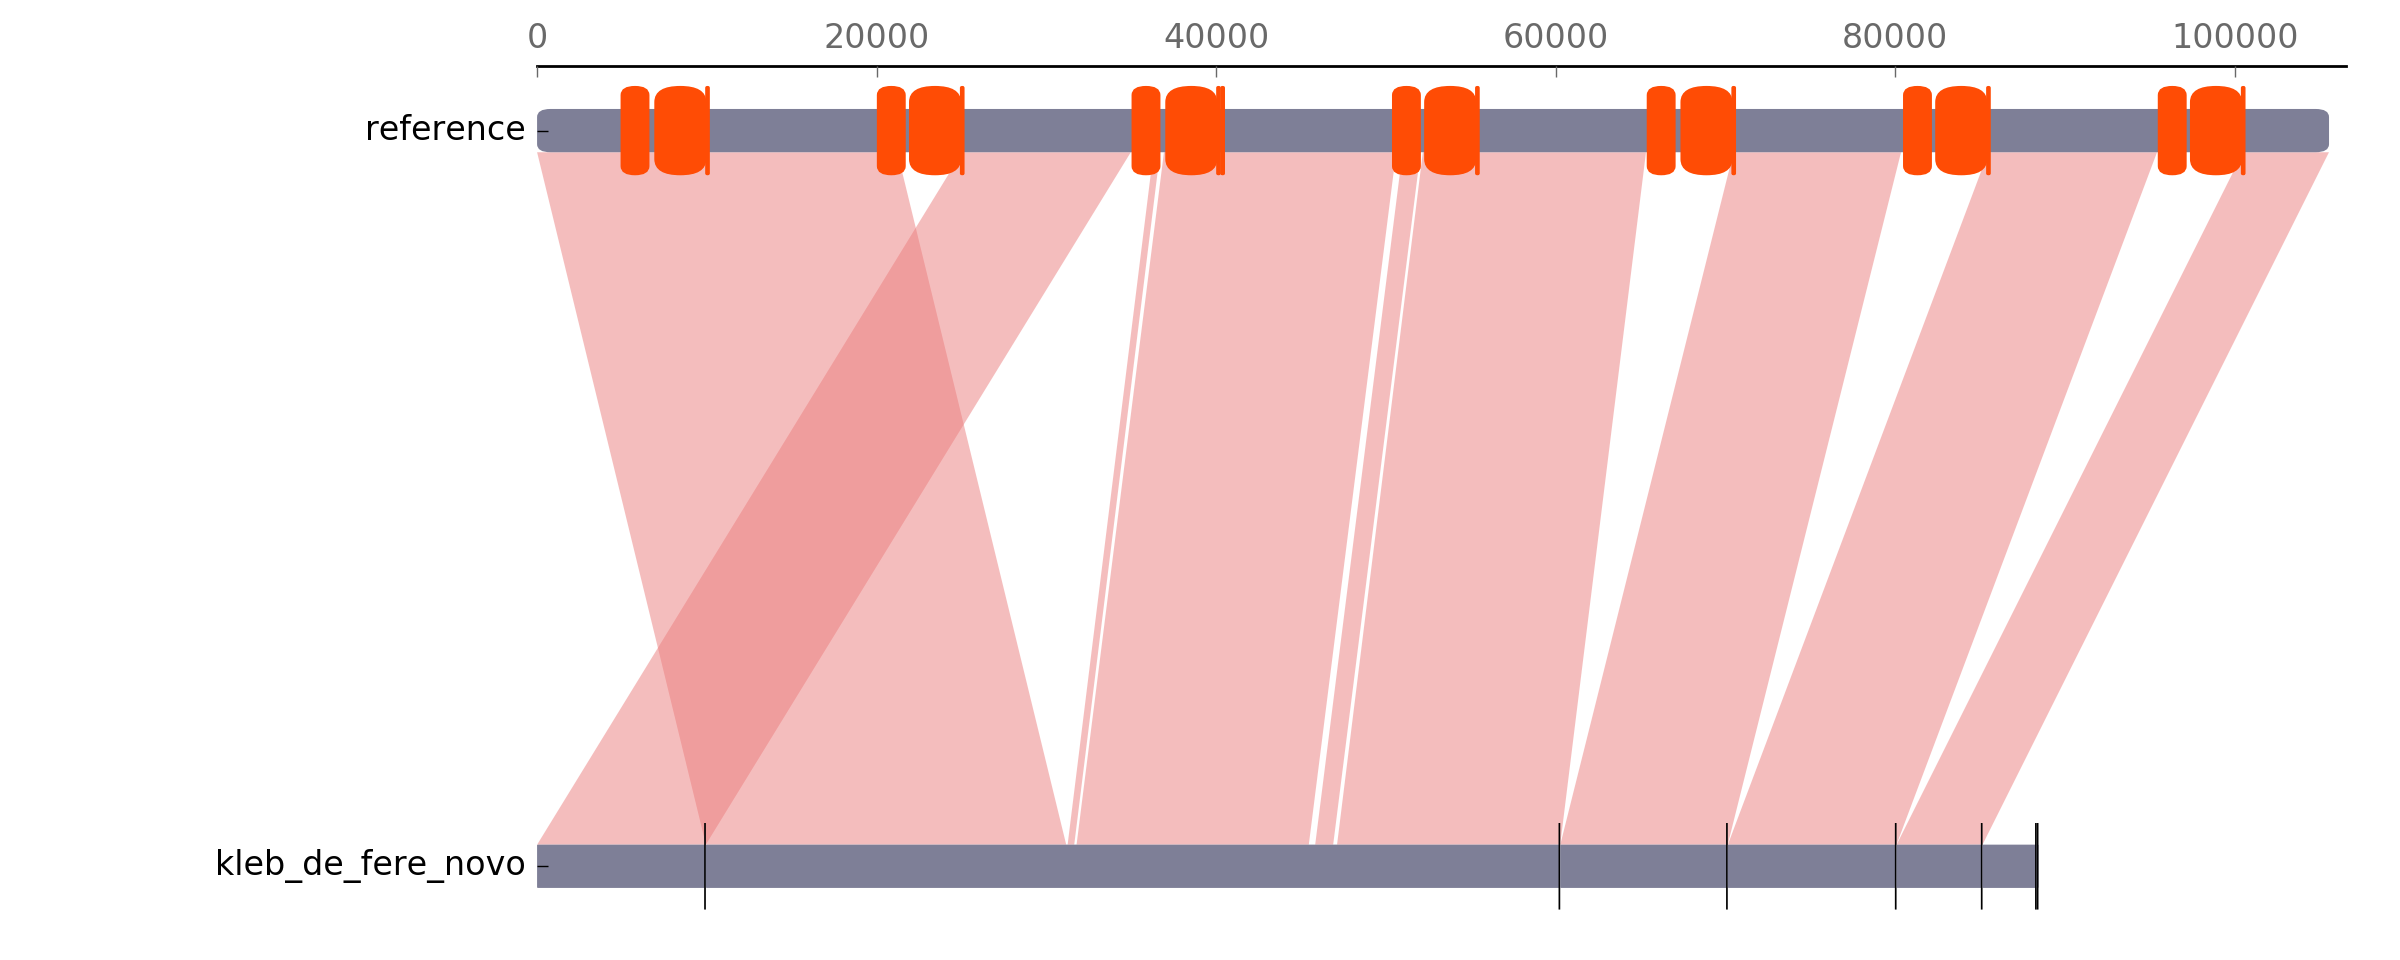
\includegraphics[width=1.2\columnwidth]{../../../NAR_riboSeed/riboFigs/PrettyMauve}
    \caption{Representative Mauve output describing the results of riboSeed assemblies of simulated reads generated by pIRS from the concatenated \textit{E. coli} Sakai artificial chromosome. Red regions represent rRNA coding sequences, vertical black lines indicate boundaries between assembled contigs, and shading represents synteny. From top to bottom: artificial reference chromosome; rDNA clusters (red bars); \textit{de fere novo} assembly and \textit{de novo} assembly (both using \textit{E. coli } MG1655 as the reference). riboSeed's \textit{de fere novo} method assembles 4 of 7 rDNA regions, but the \textit{de novo} assembly recovers no rDNA regions correctly.
}
\label{fig:artificial}
\end{figure}


\input{../../../NAR_riboSeed/main_tex/resartificial}



\subsection*{Effect of reference sequence identity on riboSeed performance}

\input{../../../NAR_riboSeed/main_tex/ressimread1}
\input{../../../NAR_riboSeed/main_tex/figdegen}
\input{../../../NAR_riboSeed/main_tex/ressimread2}
\input{../../../NAR_riboSeed/main_tex/figcolikleb}

\subsection*{Simulated reads with \textit{E. coli} and \textit{K. pneumoniae} genomes}

\input{../../../NAR_riboSeed/main_tex/ressimread3}

\subsection*{Benchmarking against hybrid sequencing and assembly}

\input{../../../NAR_riboSeed/main_tex/reshybrid}
\input{../../../NAR_riboSeed/main_tex/tabsnps}

\subsection*{Case Study: Closing the assembly of \textit{S. aureus} UAMS-1}

\input{../../../NAR_riboSeed/main_tex/resuams1}

\subsection*{Benchmarking against GAGE-B Datasets}

\input{../../../NAR_riboSeed/main_tex/tabbenchmark}
\input{../../../NAR_riboSeed/main_tex/resbenchmark}

\section*{Discussion}
\input{../../../NAR_riboSeed/main_tex/discussion}

\section*{Conclusions}
\input{../../../NAR_riboSeed/main_tex/conclusion}

\end{linenumbers}
\baselineskip13pt

\section*{List of abbreviations}
rDNA: DNA region coding for ribosomal RNA operon; rRNA: ribosomal RNA; SRA: Sequence Read Archive; ENA: European Nucleotide Archive; IG: intergenic, GAGE-B: Genome Assembly Gold-standard Evaluation for Bacteria


\section*{Competing interests}
The authors declare that they have no competing interests.

\section*{Funding}
The work was funded through a joint studentship between The James Hutton Institute, Dundee, Scotland, and the National University of Ireland, Galway, Ireland.

\section*{Authors' contributions}
NRW wrote all the bugs.

\section*{Acknowledgements}
We thank Anton Korobeynikov for his recommendations on optimizing SPAdes. Yoann Augagneur, Shaun Brinsmade, and Mohamed Sassi graciously provided access to the \textit{S. aureus} UAMS-1 genome sequencing data.  Additional computational resources were provided by CLIMB \cite{Connor2016}. We thank the Bioconda (\url{https://bioconda.github.io/}) community for their support.




\pagebreak
\bibliography{../../../NAR_riboSeed/riboSeed_refs}
\pagebreak

% \beginsupplement
% \section*{Supplementary Data}


% %%%% METHODS
% \input{../../../NAR_riboSeed/supp_tex/extendedmethods}
% \input{../../../NAR_riboSeed/supp_tex/keyparams}

% %%%% TABLES
% % table S1
% \input{../../../NAR_riboSeed/supp_tex/tablesrahits}
% % table S2
% \input{../../../NAR_riboSeed/supp_tex/tablecolis}
% % table S3
% \input{../../../NAR_riboSeed/supp_tex/tableaccessions}
% % table S4
% \input{../../../NAR_riboSeed/supp_tex/tablesoftware}
% % table S5
% \input{../../../NAR_riboSeed/supp_tex/tablequastpao}
% % table S6
% \input{../../../NAR_riboSeed/supp_tex/tablequastuams1}
% % table S7
% \input{../../../NAR_riboSeed/supp_tex/phylaperformance}
% \input{../../../NAR_riboSeed/supp_tex/tableperformance}

% %%%% FIGURES
% % Figure S1
% \input{../../../NAR_riboSeed/supp_tex/figsalgo}
% % Figure S2
% \input{../../../NAR_riboSeed/supp_tex/figsblast}
% % Figure S3
% \input{../../../NAR_riboSeed/supp_tex/figsartificial}
% % Figure S4
% \input{../../../NAR_riboSeed/supp_tex/figsgage}
% % Figure S5
% \input{../../../NAR_riboSeed/supp_tex/figscereus}
% % Figure S6
% \input{../../../NAR_riboSeed/supp_tex/atypical}
% % Figure S7

% \bibliographystyle{unsrt}

\end{document}




%%%%%%%%%%%%%%%%%%%%%%%%%%%%%%%%%%%%
% note about ANI and spceies boundary
% fix graph ab
% fix replicates
